%%%%%%%%%%%%%%%%%%%%%%%%%%%%%%%%%%%%%%%%%%%%%%%%%%%%%%%%%%%%%%%%%%
% Artigo segundo as normais mais atualizadas da ABNT
% Adaptado do projeto ABNTeX2 (que nao esta totalmente sincronizada com as normas da ABNT)
% Autor: Berg Dantas (bergdantas@msn.com)
%%%%%%%%%%%%%%%%%%%%%%%%%%%%%%%%%%%%%%%%%%%%%%%%%%%%%%%%%%%%%%%%%%
\documentclass[hidelinks, article,12pt,oneside,a4paper,english,brazil,sumario=tradicional]{abntex2}		
% Pacotes usados
\usepackage{times}%Usa a fonte Latin Modern
\usepackage[T1]{fontenc}%Selecao de codigos de fonte.
\usepackage[utf8]{inputenc}%Codificacao do documento
\usepackage{indentfirst}%Indenta o primeiro parágrafo de cada seção.
\usepackage{nomencl}%Lista de simbolos
\usepackage{color}%Controle das cores
\usepackage{graphicx}%Inclusão de gráficos
\usepackage{microtype}%Para melhorias de justificação
\usepackage{lipsum}%Para geração de dummy text
\usepackage[abnt-emphasize=bf,abnt-and-type=e,alf]{abntex2cite}%Citações ABNT
\usepackage{mathptmx}
\usepackage{amsfonts}
\usepackage{amsmath}
\usepackage{amssymb}
\usepackage{amsthm}
\usepackage{float}
%\usepackage[bottom=2cm,top=3cm,left=3cm,right=2cm]{geometry}
\usepackage{longtable}
%\frontmatter % As páginas após este comando e antes do comando \mainmatter, serão numeradas com algarismos romanos minúsculos.

% Para colocar a numeração das pagninas no canto superior direito 
\usepackage{blindtext}% only for dummy text
\usepackage{fancyhdr}
\pagestyle{fancyplain}% <- use fancyplain instead fancy
\fancyhf{}
\fancyhead[R]{\thepage}
\renewcommand{\headrulewidth}{0pt}

\usepackage{times}	
\renewcommand{\ABNTEXchapterfontsize}{\Large}
\renewcommand{\ABNTEXchapterfont}{\lmodern}
% ---
% PACOTES
% ---

% ---
% Pacotes fundamentais 
% ---
\usepackage{cmap}				% Mapear caracteres especiais no PDF
\usepackage{mathptmx}			% Usa a fonte Latin Modern	
%\usepackage{chngcntr}          % Sem esse a numeração ficou normal
%\counterwithin{table}{chapter} % Sem esse a numeração ficou normal
%\counterwithin{figure}{chapter} % Sem esse a numeração ficou normal
\usepackage[T1]{fontenc}		% Selecao de codigos de fonte.
\usepackage[utf8]{inputenc}		% Codificacao do documento (conversão automática dos acentos)
\usepackage{lastpage}			% Usado pela Ficha catalográfica
\usepackage{indentfirst}		% Indenta o primeiro parágrafo de cada seção.
\usepackage{color}				% Controle das cores
\usepackage{microtype} 	        % para melhorias de justificação
\usepackage{graphicx}			% Inclusão de gráficos
\usepackage[top=3cm, bottom=2cm, left=3cm, right=2cm]{geometry}
\usepackage{hyperref}
\usepackage{float}
\usepackage{amsmath}
\usepackage{lscape}
\usepackage[colorinlistoftodos,prependcaption,textsize=tiny]{todonotes}
\usepackage{caption}
\counterwithout{footnote}{chapter}
\usepackage{pdfpages}
\usepackage{enumitem}
\usepackage{nomencl} 			% Lista de simbolos
\usepackage{multirow}
\usepackage{caption}
\usepackage{subcaption}
\usepackage{longtable}
\usepackage{tikz}
\usepackage{array}
\usepackage{tikz}
\usepackage{smartdiagram}
\usepackage{forest}
\usepackage{pgfplots}
\usepackage{xcolor}
\usepackage{pgfkeys}
\usepackage{pgfplots}
\usepackage{forest}
\useforestlibrary{edges}
\usepackage{tikz}
\usetikzlibrary{matrix}
\usepackage{colortbl}
\usepackage{appendix}
\usetikzlibrary{mindmap}  % Mindmap drawing library
\usepackage{makecell} % Permite forçar mudanças de linha numa célula de uma tabela
\usepackage{multirow}
\usepackage{rotating}
\usepackage{xcolor}
\usepackage{array}
\usepackage{colortbl}
\usepackage{booktabs}
\usepackage{multirow}
\usepackage{adjustbox}

\usepackage[newfloat]{minted} % Correção dos bugs dos quadros
\usepackage{caption} % Para reduzir o espaço da legenda com a tabela (O "longtable" gerar espaços desnecessários)
\captionsetup{skip=0pt} % Para reduzir o espaço da legenda com a tabela/quadro
%% Usar também o "\vspace*{-5.5mm}" antes do "Fonte: Elaboração Própria" para diminuir o espaço 

%


% ---
		
% ---
% Pacotes adicionais, usados apenas no âmbito do Modelo Canônico do abnteX2
% ---
\usepackage{lipsum}				% para geração de dummy text
\usepackage{rotating}

% ---

% ---
% Pacotes de citações
% ---
\usepackage[brazilian,hyperpageref]{backref}	 % Paginas com as citações na bibl
\usepackage[alf]{abntex2cite}	% Citações padrão ABNT

% --- 
% CONFIGURAÇÕES DE PACOTES
% --- 

% ---
% Configurações do pacote backref
% Usado sem a opção hyperpageref de backref
\renewcommand{\backrefpagesname}{Citado na(s) página(s):~}
% Texto padrão antes do número das páginas
\renewcommand{\backref}{}
% Define os textos da citação
\renewcommand*{\backrefalt}[4]{
	\ifcase #1 %
		Nenhuma citação no texto.%
	\or
		Citado na página #2.%
	\else
		Citado #1 vezes nas páginas #2.%
	\fi}%
% ---




% Configuracoes do documento
\graphicspath{{./Figuras/}}%Images na pasta "Figuras"
\setsecheadstyle{\bfseries \normalsize \uppercase}
\setsubsecheadstyle{\normalsize \uppercase}
\setsubsubsecheadstyle{\bfseries \normalsize}
\setlrmarginsandblock{3cm}{2cm}{*}%Margens esquerda-direita
\setulmarginsandblock{3cm}{2cm}{*}%Margens cima-baixo
\checkandfixthelayout
\setlength{\parindent}{1.25cm}%paragrafo
\OnehalfSpacing%espacamento de 1,5
\setlength{\ABNTEXcitacaorecuo}{4cm}%recuo citacao direta +3

\begin{document}
\selectlanguage{brazil} % Seleciona o idioma do documento
\frenchspacing % Retira espaço extra obsoleto entre as frases.

\begin{center}
%TITULO
	\uppercase{\bfseries{Efeitos do Choque da Taxa de juros sobre setor bancário: Um Modelo Simplificado com Agentes}}
	\vspace{12pt}
\end{center}

% Títulos Alternativos

% "Impacto Regulatório no Setor Bancário: Uma Abordagem por Modelagem de Agentes"

% "Explorando a Resiliência do Setor Bancário diante de Choques Regulatórios: Uma Modelagem Baseada em Agentes"

% Explorando os Efeitos de Choques Regulatórios: Uma Modelagem Baseada em Agentes para o Setor Bancário

\begin{flushright}
%AUTOR - Pode-se contar com infinitos autores   :)
	Iuri Everson Silva Monteiro \footnote{Doutorando em Economia pelo Instituto de Economia da Universidade Federal do Rio de Janeiro (IE/UFRJ). E-mail: iurieverson@gmail.com. ORCID n°: 0000-0002-8445-2535.}
\end{flushright}



\textual
\pagestyle{simple}
\aliaspagestyle{chapter}{simple}

\noindent \textbf{Resumo}: Este artigo investiga o impacto da Taxa de juros sobre algumas variáveis do setor bancário por meio de uma abordagem de modelagem baseada em agentes. Ao adotar uma perspectiva de modelagem baseada em agentes, o artigo busca oferecer \textit{insights} valiosos sobre a complexidade das interações no setor bancário diante da mudança exógena imposta e assim contribuir para uma compreensão mais aprofundada dos desafios e oportunidades enfrentados pelas instituições financeiras. O aumento da taxa de juros teve um impacto significativo no setor bancário, impulsionando o patrimônio e a lucratividade para níveis mais altos, enquanto provocava uma diminuição temporária nas reservas e uma queda no Market share. A crescente preocupação com a gestão de riscos resultou em um aumento na provisão de perdas esperadas.

% Este artigo investiga os efeitos dos choques regulatórios no setor bancário por meio de uma abordagem de modelagem baseada em agentes. Utilizando simulações computacionais, o estudo explora como mudanças nas regulamentações impactam o comportamento dos agentes dentro do sistema bancário simples. O objetivo é compreender as dinâmicas resultantes desses choques e sua influência nas operações e desempenho dos bancos. A análise se concentra na resposta dos agentes às mudanças regulatórias, examinando possíveis efeitos sobre a estabilidade financeira, competitividade e eficiência do setor. Ao adotar uma perspectiva de modelagem baseada em agentes, o artigo busca oferecer insights valiosos sobre a complexidade das interações no setor bancário diante de mudanças regulatórias, contribuindo para uma compreensão mais aprofundada dos desafios e oportunidades enfrentados pelas instituições financeiras.

\vspace{2mm}

\noindent \textbf{Palavras-Chave}: Choque exógeno; Setor bancário; Modelo baseado em agentes

\vspace{2.5mm}

\noindent \textbf{Abstract}: This article investigates the impact of the interest rate on certain variables within the banking sector through an agent-based modeling approach. By adopting an agent-based modeling perspective, the article seeks to provide valuable insights into the complexity of interactions in the banking sector in the face of imposed exogenous change and thereby contribute to a deeper understanding of the challenges and opportunities faced by financial institutions. The increase in the interest rate had a significant impact on the banking sector, driving up both assets and profitability, while causing a temporary decrease in reserves and a decline in market share. The growing concern over risk management led to an increase in expected loss provisions.

\vspace{2mm}

\noindent \textbf{Keywords}: Exogenous Shock; Banking sector; Agent-based model



\section{Introdução}
\label{secIntroducao}
\normalsize
% TEXTO DA INTRODUCAO

Na perspectiva convencional, mainstream, os bancos comerciais são compreendidos apenas como intermediários das relações dos agentes deficitários e superavitários, além disso, com a finalidade de corrigir as assimetrias de informações dos atores econômicos, tais desequilíbrios são: custos de transação, de informações e de verificação dos riscos. Além disso, essas instituições são consideradas incapazes de influenciar os rumos da economia através de suas decisões (Princípio da neutralidade), visto que são inaptas para gerar liquidez, o que permitiria intervir nas escolhas de alocação de renda dos agentes \cite{paula2013financiamento}.

Entretanto, a visão do sistema bancário como apenas intermediadores neutros é totalmente equivocada. Os bancos comerciais representam um dos ramos mais dinâmicos e complexos do Sistema Financeiro, sendo um dos principais agentes que colaboram para a riqueza do país.  \citeonline{oliveira2014paula} e \citeonline{paula2013financiamento} ressaltam que essas instituições financeiras são ativas dentro de um economia, já que afetam a dinâmica da acumulação capitalista através do financiamento de investimentos e no processo endógeno de criação de moeda escritural.

Keynes apresentou indícios da importância do sistema bancário para a economia capitalista nas seguintes passagens “(...) Em geral, os bancos detêm a posição-chave na transição de uma escala de atividade mais baixa para uma mais alta (...)” \cite[p.668]{keynes1937alternative} e “(...) Pela escala e pelos termos em que está disposto a conceder empréstimos, o sistema bancário está em condições, sob um regime de moeda representativa, de determinar – em linhas gerais – a taxa de investimento do mundo empresarial. (...)” \cite[vol. 1, p.668]{keynes1930treatise}. 

Tal fato evidencia a função ativa que os bancos exercem na economia. Por um lado, estimulando o ciclo de expansão através da alta liquidez nas fases de expectativas otimistas e ampliação dos negócios e, por outro, aumentando o nível de preferência pela liquidez e racionamento de crédito na fase de deterioração das expectativas otimistas. Em outras palavras, desempenham o dúbio papel de incentivador do crescimento econômico e impulsionador da instabilidade financeira. \citeonline{terra2014sistema} indica que o setor bancário tem como principal característica sua natureza pró-cíclica e indutora do ciclo, assim, quanto mais fragilizada for a economia maior será a crise. Os impactos de choques exógenos no setor bancário podem ser profundos e abrangentes, afetando não apenas a operação diária das instituições financeiras, mas também reverberando na economia como um todo. Quando confrontados com mudanças nas regulações e no cenário imposto, os bancos frequentemente ajustam suas estratégias de investimento e concessão de crédito para se adequarem às novas exigências legais.

É crucial compreender que as instituições financeiras, em momentos de crises, têm a tendência de buscar ativos mais líquidos em seus portfólios, como moeda e títulos do governo, a fim de garantir uma posição mais segura diante da volatilidade do mercado \cite{junior2019preferencia} \cite{paula1998comportamento}. Esse movimento reflete uma busca pela redução de riscos e pela proteção contra potenciais perdas financeiras. No entanto, quando choques regulatórios são introduzidos, o ambiente macroeconômico mudam, e os bancos precisam ajustar suas estratégias para cumprir as novas normativas. Os choques regulatórios no setor bancário, como, por exemplo, Choque de Juros desempenham um papel crucial na modelagem e na dinâmica financeira das instituições financeiras. Essas mudanças nas regulamentações têm implicações profundas que reverberam em diferentes aspectos do sistema bancário e da economia como um todo.

O Choque de Juros, por sua vez, tem implicações diretas nos custos de financiamento para os bancos e, por extensão, para os mutuários. Aumentos nas taxas de juros podem resultar em custos mais elevados para os empréstimos, desencorajando a tomada de crédito e impactando os investimentos. Por outro lado, reduções nas taxas de juros podem estimular a demanda por crédito, mas também podem criar desafios para os bancos em termos de margens de lucro.

Em resumo, os choques regulatórios no setor bancário têm um impacto multifacetado, influenciando a oferta de crédito, os custos de financiamento, a liquidez do sistema bancário e a gestão de riscos. A interconexão desses fatores destaca a importância de um equilíbrio cuidadoso na formulação e implementação de regulamentações, visando promover a estabilidade financeira e estimular o crescimento econômico de maneira sustentável. Justifica-se a utilização do exercício empírico modelagem baseada em agentes, por incorporar aspectos que fazem parte de sistemas complexos, como a heterogeneidade (empresas com tamanhos diferentes), autonomia, interações locais (empresas pequenas seguires as decisões das empresas líderes), racionalidade limitada (os agentes não possuem todas as informações disponíveis) \cite{miller2009complex} \cite{lima2014arcaboucco} \cite{putriani2020exploration} \cite{teixeira2016bank}. 

Um agente é um indivíduo ou objeto autônomo com particularidades e ações inserido numa simulação computacional \cite{wilensky2015introduction} \cite{alaliyat2019comparison}. Dessa forma, a modelagem baseada em agentes é fundamentada na ideia de que o mundo pode ser modelado mediante ao estabelecimento de múltiplos agentes distribuídos seguindo regras simples de comportamento e com a finalidade de observar os resultados da interação entre eles \cite{alaliyat2019comparison}. Em outras palavras, essa ferramenta computacional possui a capacidade de descrever economias artificiais, através da criação de um conjunto de entidades autônomas, os agentes, que interagem um com os outros dentro desse ambiente computacional. Além desse ambiente de interação, é definido uma coleção de características, regras comportamentais próprias e a comunicação e aprendizagem dessa população de objetos.  


\section{Revisão de Literatura}

Esta seção apresenta uma análise de estudos anteriores que compartilham similaridades com a proposta deste trabalho, sublinhando a importância de tal discussão. Ressalta-se, desde já, que este não é um estudo exaustivo. Não é surpreendente o aumento rápido no número de estudos que empregam \textit{ABM's} para analisar sistemas bancários e financeiros nos últimos anos, tornando evidente que esta revisão da literatura não é de forma alguma minuciosa e não pode dar conta de todo o trabalho passado e em curso nesta área.

O artigo de \citeonline{chan2017abba} apresenta uma abordagem inovadora na análise de riscos no sistema bancário, destacando a importância de incorporar a heterogeneidade e o comportamento adaptativo dos bancos em resposta a choques e mudanças nas condições de negócios e regulatórias. O modelo proposto, ABBA, baseado em agentes, permite uma análise detalhada das interações no sistema bancário, incluindo a formação de redes interbancárias. Ao considerar as decisões de negócios dos bancos, como pagamento de dividendos, expansão de crédito e ajustes dinâmicos do balanço, o ABBA oferece insights valiosos sobre o impacto das mudanças regulatórias na solvência, liquidez e interconectividade. 

A abordagem baseada em agentes enriquece as opções disponíveis para os participantes do mercado, possibilitando a formulação de políticas regulatórias mais informadas e a avaliação de riscos em cenários hipotéticos. Simulações numéricas realizadas demonstram a utilidade do ABBA em capturar a dinâmica do sistema bancário tradicional e sua capacidade de ser estendido para modelar riscos em sistemas bancários mais complexos. 


O artigo de \citeonline{dadej2020agent} apresenta um modelo do setor bancário baseado em agentes, que inclui três tipos distintos de agentes: famílias, mutuários e bancos. As famílias fornecem fundos ao setor bancário por meio de depósitos e estão sujeitas a mudanças estocásticas em sua escolha de banco. Os mutuários representam a principal fonte de demanda por liquidez no sistema, utilizando-a para investimentos, resultando em possíveis inadimplências de empréstimos. Por fim, os bancos atuam como intermediários entre os dois tipos de agentes anteriores e gerenciam seus balanços de forma simplificada. 

O estudo incorpora choques em três variáveis-chave: o índice de reservas mínimas, a probabilidade de inadimplência e o índice de adequação de capital. Em sua conclusão, o artigo destaca a utilidade do modelo proposto para avaliar os impactos de choques exógenos adversos no setor bancário e seu risco sistêmico. Além disso, ressalta a atratividade da abordagem baseada em agentes como uma alternativa viável aos modelos mais convencionais, oferecendo uma representação mais holística da economia, a capacidade de incorporar fatos estilizados de forma clara e uma interpretabilidade aprimorada.


O artigo de \citeonline{lima2014arcaboucco} tem como objetivo principal descrever a concepção e a construção de um arcabouço computacional voltado para o estudo do setor bancário por meio de modelos baseados em agentes. A metodologia empregada se baseia em uma versão iterada do modelo Diamond-Dybvig, incorporando agentes de diferentes tipos, como instituições financeiras, firmas, depositantes e bancos centrais. O arcabouço é exemplificado através de aplicações envolvendo questões como seguro de depósitos, emprestador de última instância, mercado interbancário, risco de crédito e requerimento de capital.

Os resultados obtidos demonstram que o arcabouço construído pode ser aplicado satisfatoriamente em diferentes situações, apesar de utilizar protótipos conceituais não calibrados com dados reais. Contudo, devido à complexidade dos problemas abordados, o arcabouço e os exemplos apresentados são considerados simplificados demais para serem diretamente aplicáveis no mundo real, sendo vistos como passos intermediários para modelos mais aprofundados. 


O artigo de \citeonline{khan2014impact} tem como objetivo principal analisar o impacto das variações nas taxas de juros sobre a rentabilidade dos bancos comerciais no Paquistão, utilizando dados financeiros de quatro grandes bancos entre os anos de 2008 e 2012. O estudo destaca a importância da eficiência do setor bancário para o crescimento econômico e a estabilidade macroeconômica, especialmente em um contexto onde o \textit{spread} de juros no Paquistão está em ascensão, influenciando a poupança e o investimento. 

A metodologia empregada consiste na utilização do método de correlação de Pearson para examinar a relação entre as taxas de juros e a rentabilidade dos bancos comerciais. Os resultados revelam uma correlação forte e positiva entre as taxas de juros e a lucratividade dos bancos, indicando que mudanças nas taxas de juros impactam diretamente a rentabilidade dos bancos. Na conclusão, o estudo destaca a dependência da rentabilidade dos bancos em relação às taxas de juros, ressaltando que a política monetária desempenha um papel crucial nesse aspecto. 

O artigo de \citeonline{peng2003impact} propõe uma avaliação do impacto do aumento das taxas de juros sobre os lucros dos bancos em Hong Kong. O estudo se concentra na relação empírica entre a taxa de juros de mercado, a margem de juros líquida dos bancos e o índice de empréstimos classificados, que determina as provisões.

Os principais resultados destacam que o lucro antes de impostos dos bancos de varejo em Hong Kong é principalmente impulsionado por mudanças na margem de juros líquida e no encargo líquido das provisões. Durante o período de estudo, observou-se que o aumento no spread sobre a taxa de juros comprimiu a margem de juros líquida e deteriorou a qualidade dos ativos bancários. Esses resultados sugerem que as mudanças nas taxas de juros, especialmente o spread sobre a taxa de juros, desempenham um papel significativo na determinação dos lucros dos bancos em Hong Kong. 








\section{Metodologia}

O presente modelo é inspirado nos trabalhos de \citeonline{chan2017abba} e \citeonline{dadej2020agent}. Neste modelo baseado em agentes para o setor bancário enfoca a estrutura e os processos que regem a interação entre os diversos agentes envolvidos. Neste modelo, os agentes principais são as Famílias depositantes, os Mutuários e os Bancos, cada um desempenhando papéis cruciais no funcionamento do sistema. A metodologia detalhará como esses agentes são definidos, como interagem e como são modelados seus comportamentos individuais e coletivos. Isto é, a descrição das regras de tomada de decisão, a atribuição das características e preferências, bem como a dinâmica das transações financeiras e empréstimos. Ao delinear esses aspectos metodológicos, o modelo busca proporcionar uma simples representação da dinâmica do setor bancário. 

Conforme supracitado, existem três tipos de agentes: Famílias $(f = 1, 3,... F)$, Mutuários $(m = 1, 2, 3... M)$ e os Bancos $(b = 1, 2, 3... B)$. Os agentes iniciam as decisões em tempo discreto $(t = 1, 2, 3,... T)$. Primeiramente, as famílias desempenham o papel de fornecedores de fundos por meio de depósitos, os quais podem ser retirados da mesma maneira. Em segundo lugar, há os Mutuários que solicitam empréstimos para financiar projetos de investimento de natureza incerta. Por fim, as Instituições bancárias, que são os mais complexos devido às suas múltiplas regras e funções, atuam como intermediários entre as famílias e os Mutuários. Eles concedem empréstimos à esses últimos utilizando os fundos obtidos por meio dos depósitos das famílias, enquanto gerenciam o risco associado a essa atividade.

A ausência de certas características impede que esses agentes sejam considerados completos em termos de suas características como agentes. Essas características ausentes incluem heterogeneidade, capacidade de ajustar suas ações, responsividade e autonomia. Dentro do grupo de agentes mencionados, os bancos são considerados agentes completos de acordo com esses critérios, enquanto as famílias carecem de autonomia e os mutuários não demonstram nem autonomia nem capacidade adaptativa.

Vale lembrar que se trata de um "\textit{Toy model}", ou seja, um modelo simplificado e de natureza conceitual, projetado para explorar os princípios básicos e fundamentais de um sistema complexo, neste caso, o setor bancário. Ao simplificar as características dos agentes, o modelo se torna mais fácil de entender e analisar, permitindo uma exploração mais clara dos fenômenos essenciais que regem o sistema bancário. Portanto, embora essas ausências possam limitar a precisão do modelo em replicar comportamentos individuais complexos, elas são aceitáveis dentro do contexto de um \textit{Toy model}, onde o objetivo principal é ganhar uma compreensão ampla e simplificada do sistema em questão.

\subsection{Mecanismo de Interação}

\subsubsection{Famílias}


Na etapa inicial da simulação, cada família é atribuída a um dos bancos disponíveis através de uma distribuição aleatória uniforme. Cada depósito $(d_{f_{t}})$ tem um valor fixo que permanece constante ao longo da simulação. As famílias não têm capacidade de influenciar os bancos, portanto, recebem taxas de juros dos depósitos $(j^{d})$ determinadas pelos próprios bancos. Elas não reinvestem os juros ganhos, optando por consumi-los imediatamente. Posteriormente, as famílias podem optar por mudar de banco com uma certa probabilidade estabelecida.

A probabilidade de uma família mudar de banco $(mb)$ é determinada de forma exógena para cada família, selecionada aleatoriamente a partir de uma distribuição uniforme $U(mb_{min}$, $mb_{max})$. No entanto, há uma única exceção que permite a modificação das probabilidades atribuídas. Isso ocorre quando o banco no qual uma família depositou seus fundos apresentou retornos negativos durante o período anterior. Nesse caso, a probabilidade inicial de mudança é aumentada por um valor especificado exogenamente. É importante salientar que essa regra não visa simular corridas bancárias, mas sim entender como os depositantes reagem diante da incerteza em relação ao futuro do banco.

\subsubsection{Mutuários}

Os tomadores de empréstimos estão utilizando os fundos provenientes das famílias, intermediados pelos bancos, para investir em projetos de alto risco. Cada tomador de empréstimo é caracterizado por três atributos distintos, os quais são definidos no início da simulação e são calculados endogenamente. Estes incluem a probabilidade de inadimplência do tomador de empréstimo $(pd_{m_{t}})$ durante cada período da simulação, o valor do empréstimo $(l_{m_{t}})$ e o banco do qual o empréstimo foi adquirido. A probabilidade de inadimplência é atribuída aleatoriamente a partir de uma distribuição uniforme $U(pd_{m_{t}}min$, $pd_{m_{t}}max)$. Outros atributos incluem a ponderação do risco na carteira de empréstimos do banco e o custo de capital imposto pelo banco.

A fórmula para os bancos cotarem o custo de capital é apresentada na Equação \ref{eq:custo_capital}. Onde $m_{m}$ é Margem imposta pelo banco ao empréstimo ou o prêmio de risco dos empréstimos, $r_{free}$ é a Taxa de retorno livre de risco, $pd_{m_{t}}$ é a Probabilidade de Default e $rr$ é a Taxa de recuperação. 

\begin{equation} \label{eq:custo_capital}
r_{m} = \frac{(1 + (1+m_{m})*r_{free}) - pd_{m_{t}} * rr}{1 - pd_{m_{t}}}
\end{equation}

\begin{equation} \label{eq:peso_risco}
rw_{m} = f(pd_{m_{t}}) = 0,5 + 5*pd_{m_{t}} 
\end{equation}

Já a Equação \ref{eq:peso_risco} demonstra o preso de risco potencial de um mutuário em uma carteira de empréstimo que está em função da probabilidade de inadimplência.  

\subsubsection{Instituições bancárias}

Os bancos são os elementos mais complexos do modelo. Eles devem adquirir depósitos, utilizá-los para financiar empréstimos arriscados e, ao mesmo tempo, preparar-se para potenciais perdas. Além disso, os bancos devem calcular a quantidade de capital próprio e de reservas necessárias para cumprir os requisitos regulamentares mínimos de capital e reservas. As reservas bancárias ($RES_{banco_{t}}$) e a Taxa mínima de reserva ($MMR_{t}$) no BC são calculadas, respectivamente, conforme as Equações \ref{eq:reservas} e \ref{eq:MRR}. 

\begin{equation} \label{eq:reservas}
RES_{banco_{t}} = \biggl(\sum_{l \in L_{banco_{t}}} l_{m_{t}} * r^{l}\biggl) - \biggl(\sum_{d \in D_{banco_{t}}} d_{f_{t}} * r^{d}\biggl)+ \bigtriangleup EL_{banco_{t}} 
\end{equation}

\begin{equation} \label{eq:MRR}
RES_{banco_{t}} > MMR_{t} *  \sum_{d \in D_{banco_{t}}} d_{m_{t}} 
\end{equation}

Na qual, $L_{banco_{t}}$ é o conjunto de empréstimos solventes na carteira de um banco no período $t$, $l_{m_{t}}$ é o valor do empréstimo específico de um mutuário qualquer, $r^{l}$ é a taxa de juros paga pelo empréstimo, $D_{banco_{t}}$ é o conjunto dos depósitos contidos em um determinado banco, $d_{f_{t}}$ é o valor do depósito específico de uma família qualquer, $r^{d}$ é a taxa de juros paga pelo depósitos e $\bigtriangleup EL_{banco_{t}}$ é a variação da provisão das perdas esperadas. 

Vale ressaltar que o $MMR_{t}$ é controlado externamente e está sujeito a choques. Quando as reservas de um banco caem abaixo do limite mínimo exigido, ele é obrigado a vender seus empréstimos ($ve_{banco}$) a um preço substancialmente menor, pois não pode oferecer descontos para aumentar sua liquidez. No modelo, os empréstimos vendidos não são adquiridos por outros 

A Provisão das perdas esperadas é calculada de acordo com a Equação \ref{eq:EL}.     

\begin{equation} \label{eq:EL}
EL_{banco_{t}} = \sum_{l \in L_{banco_{t}}} l_{m_{t}} * pd_{m_{t}} * (1 - rr)
\end{equation}

O Patrimônio Líquido deve está de acordo com o índice de Adequação de Capital ($CAR_{t}$):

\begin{equation} \label{eq:CAR}
E_{banco_{t}} > CAR_{t} *  \biggl(\sum_{l \in L_{m_{t}}} l_{m_{t}} * rw_{m}\biggl) 
\end{equation}

A demonstração de resultado do banco se utiliza da Receita ($REV_{banco_{t}}$), do Custo ($Cus_{banco_{t}}$) e da Renda ($REN_{banco_{t}}$), Equação \ref{eq:renda}. Ela é adicionada ao patrimônio líquido no final do período. 

\begin{equation} \label{eq:renda}
REN_{banco_{t}} = REV_{banco_{t}} - Cus_{banco_{t}}
\end{equation}

A Equação \ref{eq:receita} apresenta o modo de calculo da Receita que advém principalmente dos juros cobrados sobre empréstimos. 

\begin{equation} \label{eq:receita}
REV_{banco_{t}} = \sum_{l \in L_{banco_{t}}} l_{m_{t}} * r^{l}_{t-1} + RES_{banco_{t-1}} * r_{free_{t-1}}   
\end{equation}

Já o Custo é calculado na Equação \ref{eq:custo}. Onde $m_{f}$ é o prêmio de risco declarado exogenamente para as famílias a fim de aplicarem para compensar a maior volatilidade associada a depositar dinheiro em bancos em comparação com a posse de dinheiro ou títulos do tesouro.

\begin{equation} \label{eq:custo}
Cus_{banco_{t}} = \sum_{d \in D_{banco_{t}}} d_{m_{t}} * \biggl[r_{free_{t}} * (1 + m_{f})\biggl]
\end{equation}


\subsubsection{Processo de simulação}

O início do período é marcado pelo processo em que os bancos iniciam a formação de suas carteiras de empréstimos. Durante essa etapa, eles determinam o montante máximo que podem emprestar, considerando as reservas mínimas e os requisitos de capital adequado, os quais são estabelecidos previamente, conforme a Equações \ref{eq:potencial_emprest} e \ref{eq: potencial_emprest2}.

\begin{equation} \label{eq:potencial_emprest}
min \biggl[\biggl((1- MMR_{t}) * \sum_{d \in D_{banco_{t}}} d_{f_{t}}\biggl) \hspace{1.5mm} , \hspace{1.5mm} \biggl(\sum^{n=na}_{l \in L_{banco_{t}}} l_{m_{t}}\biggl)\biggl]  
\end{equation}

\begin{equation} \label{eq: potencial_emprest2}
 \left \{ \begin{array}{lll}

na =  \biggl| \biggl\{ a_{i} \in (A)^{|L_{banco_{t}}|} \hspace{1.5mm} | \hspace{1.5mm} a_{i} < E_{banco_{t}} \biggl\} \biggl| \\
\\

(A)^{|L_{banco_{t}}|} = a_{i-1} + l_{m_{t}} * rw_{m_{t}} * CAR_{t} \hbox{}
\end{array}\right. 
\end{equation}

Cada novo ciclo de simulação se inicia com as famílias alocando seus depósitos e distribuindo-os entre diversos bancos, com uma menor probabilidade de escolha para aqueles que apresentaram perdas no período anterior. Posteriormente, os empréstimos são sujeitos a inadimplência com uma probabilidade previamente definida e, mais tarde, são considerados sem valor. Além do montante principal do empréstimo, o banco também perde os juros associados. Durante esse processo, os bancos calculam as perdas decorrentes de inadimplências, o que resulta em:

\begin{equation} \label{eq:perdas_incumprim}
\biggl( \bigtriangleup \sum_{l \in L_{banco_{t}}} l_{m_{t}} * r_{m_{t-1}} \biggl) * (1 - rr)
\end{equation}

Após ajustarem os depósitos e lidarem com a inadimplência dos empréstimos, cada banco verifica se atende aos requisitos obrigatórios de reserva. Aqueles que não possuem a liquidez necessária são obrigados a vender seus empréstimos. Em seguida, os bancos calculam sua prévia demonstração de lucros e perdas para atualizar seu capital e determinar em que condição financeira estão, de acordo com os critérios estabelecidos. 


\begin{equation} \label{eq:calc_fundos_disp_empr}
min \biggl[\{AF_{banco_{t}} \in \{ ER_{banco_{t}}  \hspace{1.5mm} ,  \hspace{1.5mm} EC_{banco_{t}}  \hspace{1.5mm} |   \hspace{1.5mm}AF_{banco_{t}} > 0 \}\biggl]
\end{equation}


Se o capital do banco exceder a meta de adequação de capital, ele pode optar por distribuir dividendos, equivalentes ao excesso de capital sobre a meta estabelecida. Os bancos com liquidez suficiente continuam suas atividades de empréstimo. Os fundos disponíveis para empréstimo são calculados conforme as Equações \ref{eq:calc_fundos_disp_empr}-\ref{eq:EC}.  

\begin{equation} \label{eq:ER}
 ER_{banco_{t}} = RES_{banco_{t}} - MMR_{t} * \sum_{d \in D_{banco_{t}}} d_{f_{t}}
\end{equation}

\begin{equation} \label{eq:EC}
 EC_{banco_{t}} = \sum^{n=na}_{l \in L_{banco_{t}}} l_{m_{t}}
\end{equation}

Na qual $na$ é calculado conforme a Equação \ref{eq: potencial_emprest2}. $ER_{banco_{t}}$ e $EC_{banco_{t}}$ representam os limites máximos de fundos disponíveis, determinados pelas reservas mínimas e pelos requisitos de capital adequado, respectivamente. Adicionalmente, é calculada e estabelecida a demanda máxima disponível por liquidez, Equação \ref{eq:LA}, juntamente com os empréstimos disponíveis.

\begin{equation} \label{eq:LA}
 LA_{banco_{t}} = mim \biggl[ \sum l_{d_{t}} \hspace{1.5mm} , \hspace{1.5mm} min (AF_{banco_{t}})    \biggl]
\end{equation}

\begin{equation} \label{eq:LA2}
 \{ l_{d_{t}} \in B_{banco} \hspace{1.5mm} | \hspace{1.5mm} l_{d} = 0\}
\end{equation}

Onde $B_{banco}$ representa os mutuários associados a um banco específico, e $l_{d_{t}}$ é a demanda de empréstimo, com $0$ indicando que o mutuário não está buscando financiamento. Quando $l_{d_{t}} > min (AF_{banco_{t}})$, os mutuários elegíveis recebem empréstimos de forma aleatória. É importante notar que, sem perda de generalidade, a participação de mercado de um banco específico geralmente permanece constante, impedindo assim a competição direta entre os bancos. No entanto, existem outros mecanismos descritos que incorporam ou simulam a concorrência de outras maneiras.

Por fim, são estabelecidos os valores das condições iniciais, conforme na Tabela \ref{Tab:cond_eco_art}.

\renewcommand\LTcaptype{table}
\begin{center}
\begin{longtable}{lc}
\caption{Condições iniciais da economia artificial.} \label{Tab:cond_eco_art} \\
\hline
\rowcolor[gray]{.9}
\multicolumn{1}{l}{\textbf{Condições Iniciais}} & \multicolumn{1}{c}{\textbf{Valores}} \\ \hline 
\endfirsthead
\multicolumn{2}{l}%
{{\bfseries \tablename\ \thetable{} -- Continuação da página anterior}} \\
\hline
\hline
\rowcolor[gray]{.9}
\multicolumn{1}{l}{\textbf{Condições Iniciais}} & \multicolumn{1}{c}{\textbf{Valores}}  \\ \hline 
\endhead

\hline 
\multicolumn{2}{r}{{Continuação na página seguinte}} \\ \hline
\endfoot

\hline \hline
\endlastfoot

  Número de períodos ($t$)  & 300  \\
  Número de Famílias ($f_{n}$)  & 1000  \\
  Número de Mutuários ($m_{n}$)  & 2000  \\
  Número de Bancos ($b_{n}$)  & 10  \\
  Patrimônio do banco ($E_{banco_{t}}$)  & 40  \\
  Valor do depósito ($d_{f_{t}}$) & 1 \\
  Taxa de Retorno livre de risco ($r_{free}$) & 0.125 \\
  Juros do empréstimos ($r^{l}$) & 0.02 \\
  Juros do depósitos ($r^{d}$) & 0.125 \\
  Índice de adequação de capital ($CAR_{t}$) & 0.08 \\
  Índice de reserva mínima ($MRR_{t}$) & 0.035 \\
  Margem para os depósitos ($m_{f}$) & 0.1 \\
  Margem de empréstimo ($m_{m}$) & 0.9 \\
  Taxa de recuperação ($rr$) & 0.4 \\
  Probabilidade mínima de mudar de banco $(mb_{min})$ & 0.01 \\
  Probabilidade máxima de mudar de banco $(mb_{max})$ & 0.08 \\
  Probabilidade mínima de Inadimplência ($pd_{min}$) & 0.04 \\
  Probabilidade máxima de Inadimplência ($pd_{max}$) & 0.08 \\
  Venda de emergência ($ve_{banco}$) & 0.8 
\end{longtable}

\vspace{-5mm}
Fonte: Elaboração Própria

\end{center}
 
Por fim, são estabelecidos dois cenários exogenamente, com a finalidade de auferir os impactos do aumento da taxa de juros nas variáveis bancárias. No cenário base do funcionamento do sistema bancário, sem nenhum efeito exógeno, os bancos operam de acordo com suas políticas internas e condições de mercado regulares. No segundo cenário, com o choque do aumento da taxa de juros, o sistema bancário enfrenta mudanças significativas. 



\section{Resultados}

No cenário base do funcionamento do sistema bancário, sem nenhum efeito exógeno, os bancos operam de acordo com suas políticas internas e condições de mercado regulares. As famílias depositam seus fundos nos bancos, que por sua vez utilizam esses depósitos para conceder empréstimos a mutuários elegíveis que recebem empréstimos com base em critérios pré-estabelecidos. Os bancos gerenciam suas reservas e capital de acordo com os requisitos regulamentares, mantendo um equilíbrio entre a oferta e a demanda por crédito.

A organização das variáveis em dois grupos distintos visa facilitar a análise e compreensão do desempenho da empresa. O primeiro grupo, composto por Patrimônio, Lucratividade, Dividendos e Renda, concentra-se em indicadores que refletem a saúde financeira interna da empresa. Já o segundo grupo, formado por Reservas, Receita, Provisão de Perdas Esperadas e \textit{Market Share}, abrange indicadores que demonstram a posição da empresa no mercado e sua capacidade de gerar receita.

A Figura \ref{fig:base_01} apresenta o comportamento das variáveis de Patrimônio, Lucratividade, Dividendos e Renda do Sistema bancário no caso base. O gráfico de Patrimônio exibe valores consistentes, oscilando entre 5 e 160, sugerindo uma estabilidade na posição financeira dos bancos ao longo do tempo. A lucratividade, por sua vez, apresenta uma variação mais acentuada, flutuando entre 0 e 2,7. Essa oscilação pode ser atribuída à dinâmica do mercado bancário e as estratégias de gestão adotadas pelos bancos. 

Os dividendos permanecem relativamente estáveis e em níveis baixos, indicando uma distribuição conservadora de lucros aos acionistas. Por fim, o gráfico de renda do sistema bancário mostra uma significativa oscilação ao longo do tempo, com uma leve tendência de crescimento. Essa variabilidade pode refletir a volatilidade do mercado bancário e as flutuações nas receitas e despesas dos bancos. A tendência de crescimento sugere uma expansão gradual das operações bancárias, embora sujeita a oscilações de curto prazo.



\begin{figure} [H]
\caption{Caso base: Comportamento do Patrimônio, Lucratividade, Dividendos e Renda do Sistema bancário} \label{fig:base_01}
\centering % para centralizarmos a figura

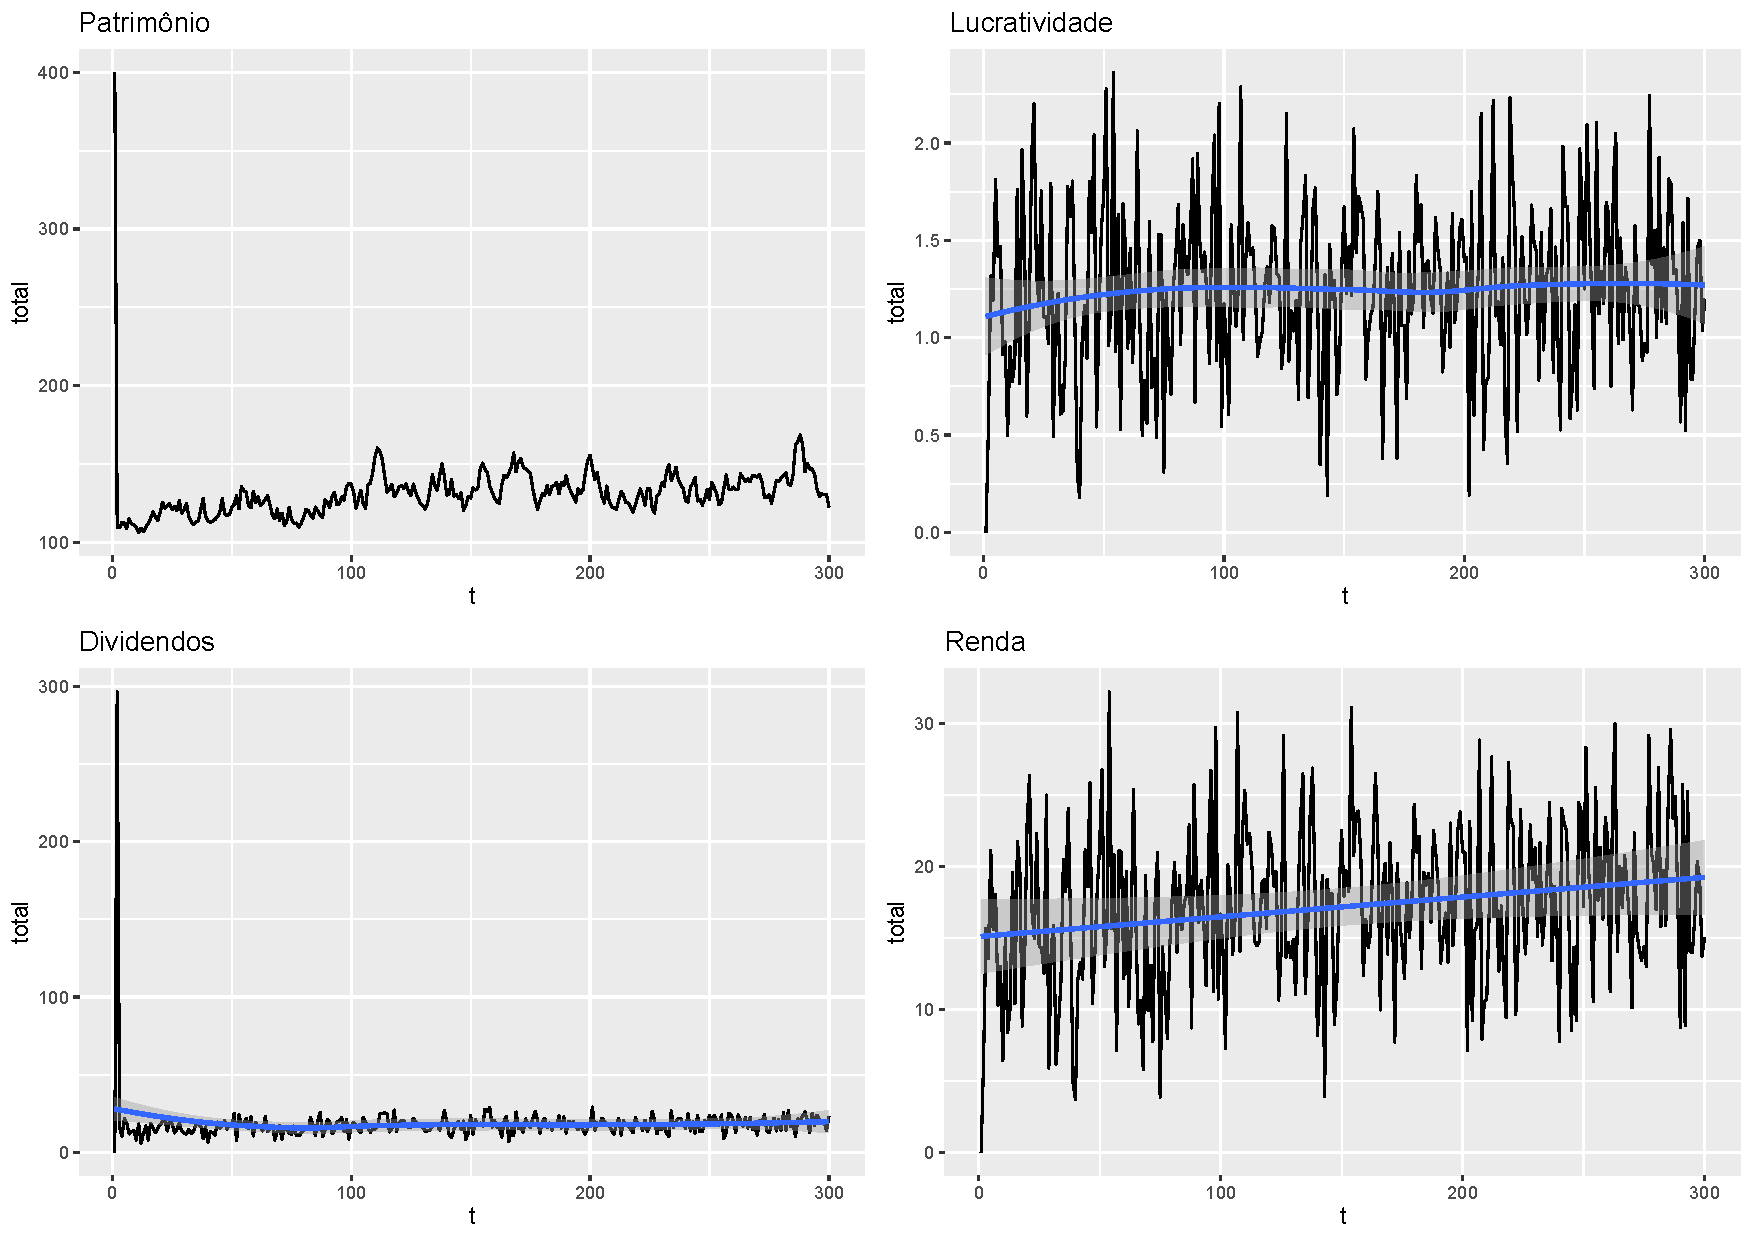
\includegraphics[width=0.9\textwidth]{figs/base_01.pdf}

Fonte: Elaboração Própria.
\label{fig:dec_var_fbcf}
\end{figure}

A Figura \ref{fig:base_02} apresenta o comportamento das variáveis de Reservas, Receita, Provisão de Perdas Esperadas e\textit{ Market Share} Sistema bancário. Em relação às reservas, observa-se uma tendência de declínio ao longo do período, atingindo um mínimo em torno do tempo 100, seguido por uma tímida recuperação. Esse padrão sugere uma possível diminuição da disponibilidade de recursos financeiros líquidos durante esse período, seguida por uma recuperação gradual. 

Quanto a receita, mantém-se numa tendência de estabilidade, dentro do intervalo de 60 a 70 ao longo do período analisado, o que indica uma consistência na geração de receita pelo sistema bancário. Por outro lado, a provisão de perdas esperadas exibe um padrão de crescimento até aproximadamente o tempo 200, seguido por um leve declínio, mas com sinais de uma recuperação subsequente. Esse comportamento pode indicar uma crescente preocupação com a gestão de riscos e a necessidade de provisionar recursos para possíveis perdas. 

Finalmente, o \textit{Market share} mostra uma grande oscilação ao longo do período, sem evidências claras de uma tendência de crescimento ou declínio. Essa volatilidade pode refletir flutuações na participação de mercado dos bancos, influenciadas por fatores como concorrência e mudanças nas preferências dos clientes.

\begin{figure} [H]
\caption{Caso base: Comportamento da Reservas, Receita, Provisão de Perdas Esperadas e Market Share Sistema bancário} \label{fig:base_02}
\centering % para centralizarmos a figura

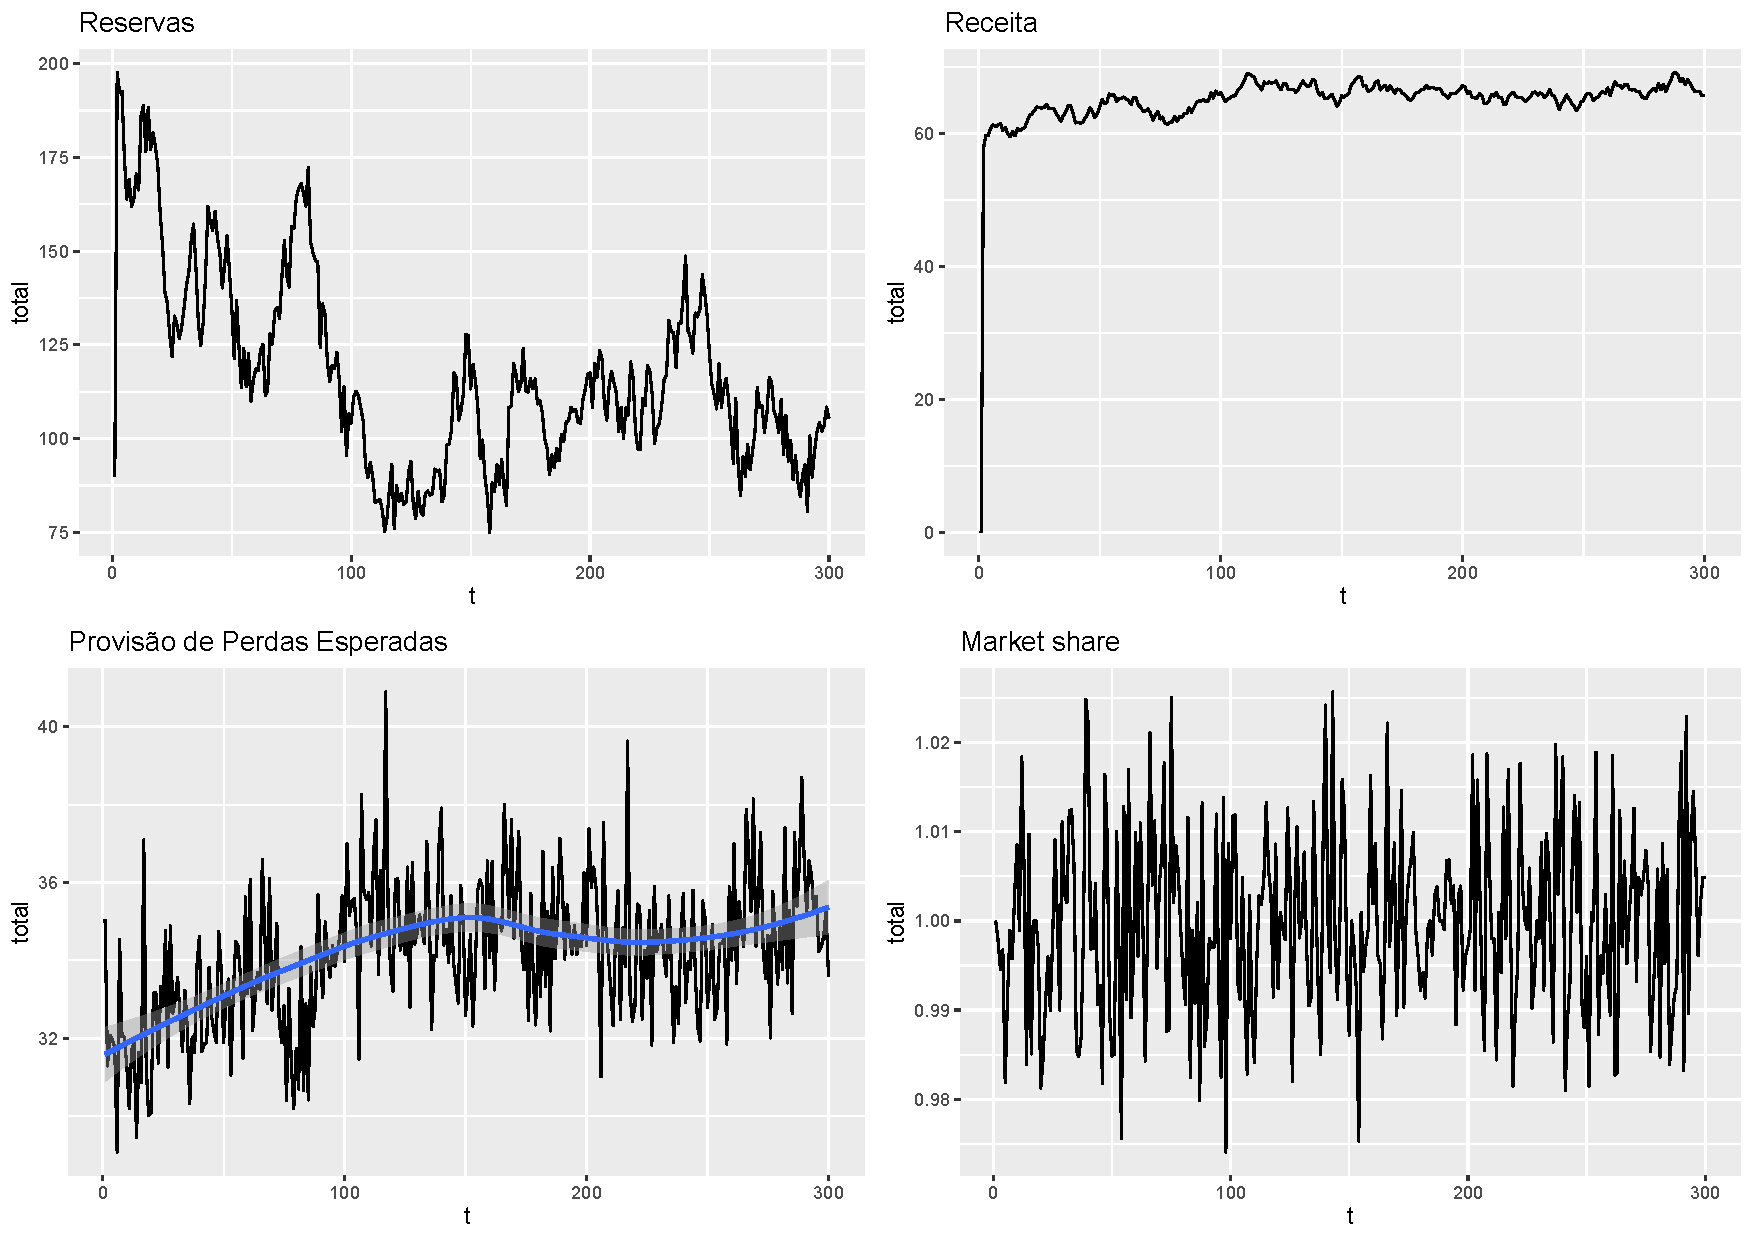
\includegraphics[width=0.9\textwidth]{figs/base_02.pdf}

Fonte: Elaboração Própria.
\label{fig:dec_var_fbcf}
\end{figure}


No segundo cenário, com o choque do aumento da taxa de juros, o sistema bancário enfrenta mudanças significativas. O aumento das taxas de juros pode resultar em uma redução na demanda por empréstimos, uma vez que os custos de empréstimo se tornam mais altos para os mutuários. Isso pode levar os bancos a ajustarem suas políticas de empréstimo e taxas de juros para compensar o aumento dos custos de captação de recursos. Além disso, o aumento das taxas de juros pode afetar a rentabilidade dos bancos e a disposição das famílias de poupar ou investir. Essas mudanças no ambiente econômico podem influenciar o comportamento dos agentes no sistema bancário e, consequentemente, a dinâmica do mercado de crédito e o desempenho financeiro dos bancos.

A Figura \ref{fig:tx_juros_01} apresenta o comportamento das variáveis do Patrimônio, Lucratividade, Dividendos e Renda do Sistema bancário após o choque da Taxa de juros. Observa-se que o patrimônio segue a mesma tendência do caso base até o período 50, quando ocorre o choque. Após esse ponto, há um aumento acentuado no patrimônio, seguido por uma manutenção constante entre os períodos 100 e 300. Esse padrão sugere que o aumento da taxa de juros teve um impacto significativo e positivo no patrimônio dos bancos podendo resultar em maiores margens de lucro para os bancos.

Já na Lucratividade, há um pico de aumento da seguido por uma ligeira queda, mas mantendo-se acima do patamar anterior ao choque. Esse padrão pode ser explicado por diversos fatores. Primeiramente, o aumento das taxas de juros pode resultar em margens de lucro mais altas para os bancos, pois eles podem cobrar taxas de juros mais elevadas em seus empréstimos enquanto os custos de captação de fundos ainda estão em níveis mais baixos, pelo menos inicialmente. Por outro lado, a ligeira queda após o pico pode ser atribuída a resposta dos concorrentes do mercado à mudança nas taxas de juros.




\begin{figure} [H]
\caption{Choque da Taxa de juros: Comportamento do Patrimônio, Lucratividade, Dividendos e Renda do Sistema bancário} \label{fig:tx_juros_01}
\centering % para centralizarmos a figura

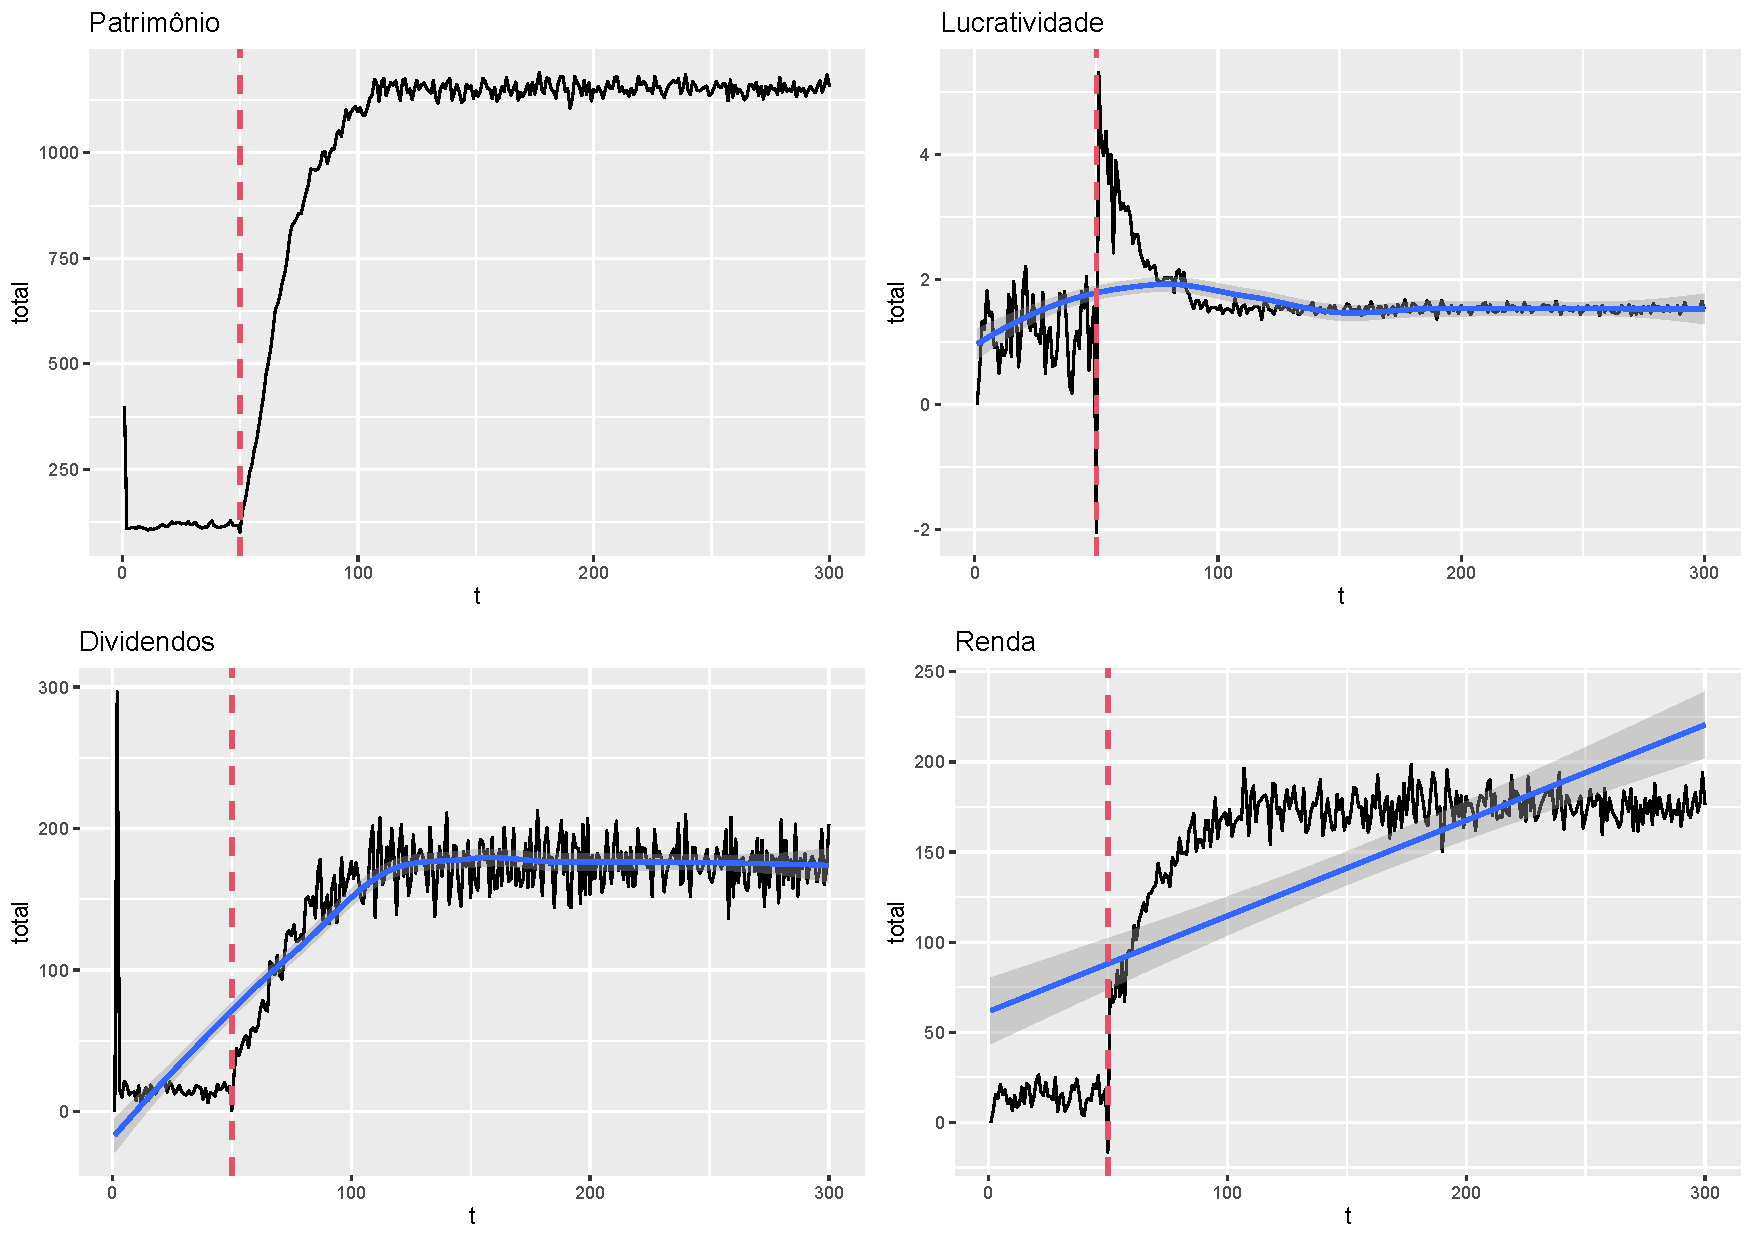
\includegraphics[width=0.9\textwidth]{figs/juros_01.pdf}

Fonte: Elaboração Própria.
\label{fig:dec_var_fbcf}
\end{figure}


Em relação aos dividendos, observa-se um aumento entre os tempos 50 e 100, seguido de uma estabilidade com oscilações subsequentes, mas sem uma tendência clara de crescimento ou decrescimento. Em relação à renda, também há um aumento após o choque, porém, após certo período, ela se mantém estável. Esses padrões podem ser explicados por diferentes fatores. O aumento dos dividendos e da renda após o choque de taxa de juros pode ser resultado do impacto positivo inicial que a mudança nas taxas teve sobre a rentabilidade dos investimentos dos bancos, levando a um aumento na distribuição de lucros aos acionistas. Após o período de aumento, a estabilidade pode refletir a estabilização da influência do choque sobre os resultados financeiros dos bancos.

No cenário do aumento da taxa de juros, Figura \ref{fig:tx_juros_02}, observa-se que após o choque, as reservas bancárias diminuem ligeiramente por um breve momento, seguidas por uma leve tendência de crescimento. Esse padrão pode ser explicado pelo impacto inicial do choque nas operações bancárias, onde as instituições podem precisar utilizar parte de suas reservas para lidar com mudanças nas condições de mercado e atender à demanda por liquidez. No entanto, a tendência de crescimento posterior pode indicar uma adaptação gradual dos bancos ao novo ambiente de taxas de juros, com estratégias de gestão de ativos e passivos sendo ajustadas para otimizar o uso das reservas e garantir a estabilidade financeira.

Por outro lado, em relação as receitas, observa-se um aumento substancial após o choque, persistindo até o tempo 100, seguido por uma estabilidade no pico. Esse aumento pode ser explicado pelos efeitos positivos do aumento das taxas de juros nas margens de lucro dos bancos, enquanto os custos de captação de fundos permanecem relativamente estáveis no curto prazo. A estabilidade subsequente no pico pode indicar uma consolidação das receitas em um novo patamar, à medida que os efeitos do choque se estabilizam e os bancos ajustam suas estratégias comerciais para o ambiente de taxas de juros alterado.


\begin{figure} [H]
\caption{Choque da Taxa de juros: Comportamento da Reservas, Receita, Provisão de Perdas Esperadas e Market Share Sistema bancário} \label{fig:tx_juros_02}
\centering % para centralizarmos a figura

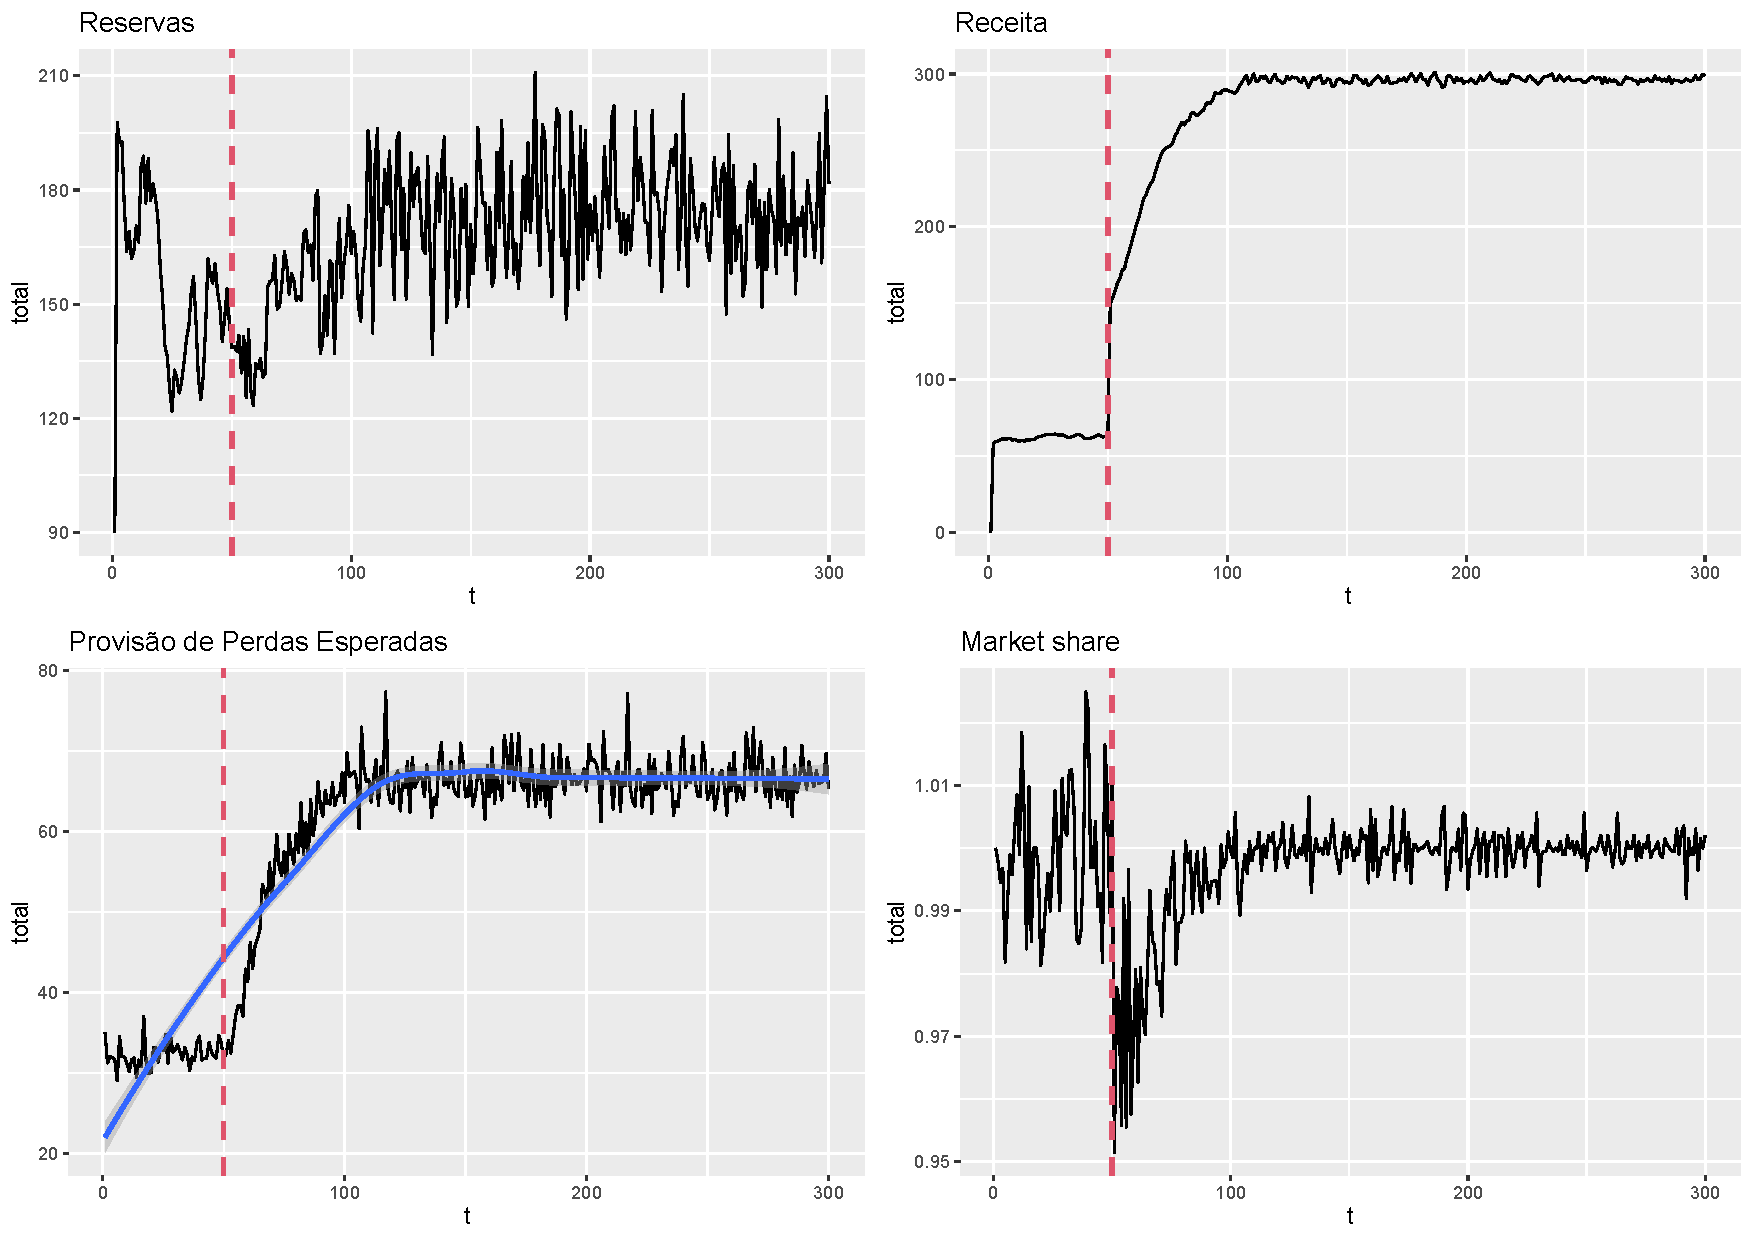
\includegraphics[width=0.9\textwidth]{figs/juros_02.pdf}

Fonte: Elaboração Própria.
\label{fig:dec_var_fbcf}
\end{figure}


Após o choque da taxa de juros, a provisão de perdas esperadas aumenta consideravelmente e se mantém relativamente constante após o período 100, sem mostrar crescimento ou decrescimento significativo. Esse aumento na provisão de perdas esperadas pode ser explicado pelo impacto das taxas de juros mais altas sobre a capacidade dos mutuários de honrar seus compromissos financeiros. 

Com taxas de juros mais elevadas, os custos de empréstimos podem aumentar, o que pode tornar mais difícil para os mutuários cumprir com seus pagamentos, resultando em um aumento nas perdas esperadas para os bancos. A estabilidade subsequente na provisão de perdas esperadas pode refletir uma acomodação das instituições financeiras a esse novo ambiente de taxas de juros, com estratégias de gerenciamento de risco sendo implementadas para mitigar os impactos adversos sobre a saúde financeira dos bancos.

Em relação ao \textit{Market share}, observa-se uma diminuição considerável após o aumento da taxa de juros, seguida por uma estabilidade no período após o tempo 100, embora em um patamar um pouco acima do que antes do choque. Essa diminuição inicial no \textit{Market share} pode ser explicada pelos efeitos das taxas de juros mais altas sobre a demanda por serviços bancários, onde os clientes podem buscar alternativas mais baratas ou adiar decisões de empréstimos devido aos custos adicionais. No entanto, a estabilidade subsequente, embora em um patamar ligeiramente superior, pode indicar uma recuperação parcial a medida que os bancos ajustam suas estratégias de mercado e adaptam seus produtos e serviços as novas condições de taxas de juros. 

Ao comparar os resultados deste estudo com as descobertas da revisão de literatura, é possível identificar várias semelhanças e complementaridades entre os dois conjuntos de resultados. Primeiramente, tanto neste estudo quanto no artigo de \citeonline{khan2014impact}, observa-se a forte influência das taxas de juros sobre a rentabilidade dos bancos.

Uma das principais conclusões de ambos os estudos é a dependência dos bancos em relação às taxas de juros e a forma como mudanças nessas taxas podem afetar diretamente a rentabilidade e a estabilidade financeira das instituições bancárias. Especificamente, neste estudo, observamos que o aumento das taxas de juros teve um impacto expressivo sobre o patrimônio e a lucratividade dos bancos, impulsionando-os para níveis mais altos inicialmente. Esses resultados estão alinhados com a forte correlação positiva entre as taxas de juros e a lucratividade dos bancos observada por \citeonline{khan2014impact}.

Além disso, os resultados deste estudo também corroboram as descobertas de \citeonline{peng2003impact} em relação ao impacto das taxas de juros sobre os lucros dos bancos. Assim como observado em Hong Kong, onde o aumento no spread sobre a taxa de juros comprimiu a margem de juros líquida e afetou a qualidade dos ativos bancários, neste estudo também observamos mudanças significativas nas variáveis financeiras dos bancos após o choque da taxa de juros. Portanto, ao comparar os resultados deste estudo com as descobertas da revisão de literatura, é possível identificar uma consistência nas conclusões em relação à influência das taxas de juros sobre a rentabilidade e a estabilidade financeira dos bancos, destacando a importância fundamental da política monetária e da eficiência do setor bancário para a saúde econômica e financeira de um país. 


\section{Considerações finais}

Nesta pesquisa, exploramos os impactos do choque da taxa de juros sobre o setor bancário por meio da modelagem baseada em agentes. Ao investigar as dinâmicas resultantes dessa mudança exógena, pudemos examinar de perto como os bancos respondem a esse tipo de perturbação e como isso afeta suas operações e desempenho. Os resultados obtidos proporcionaram uma compreensão mais profunda das interações complexas que ocorrem no setor bancário diante de mudanças nas condições do mercado financeiro.

Ao longo deste estudo, observamos que, no cenário base, os bancos operam de maneira estável, seguindo políticas internas e condições de mercado regulares. As variáveis financeiras analisadas refletiram um equilíbrio entre a oferta e a demanda por crédito, com indicadores de saúde financeira e posição de mercado demonstrando consistência ao longo do tempo.

No entanto, ao introduzir o choque do aumento da taxa de juros, observamos mudanças significativas no comportamento das variáveis do setor bancário. O aumento das taxas de juros teve um impacto expressivo sobre o patrimônio e a lucratividade dos bancos, impulsionando-os para níveis mais altos. Isso sugere uma resposta positiva inicial dos bancos ao ambiente de taxas de juros alterado, aproveitando as oportunidades de margens de lucro mais amplas.

Entretanto, também observamos efeitos adversos, como uma diminuição temporária nas reservas bancárias e uma queda no Market share, refletindo a volatilidade e os desafios que os bancos enfrentam ao se adaptarem a novas condições de mercado. Além disso, o aumento das taxas de juros levou a uma preocupação crescente com a gestão de riscos, refletida no aumento da provisão de perdas esperadas.

Apesar dessas turbulências iniciais, houve sinais de estabilização e adaptação à medida que os bancos ajustaram suas estratégias e políticas para o novo ambiente de taxas de juros. A estabilidade subsequente em várias variáveis, como receita e provisão de perdas esperadas, sugere uma capacidade de resposta eficaz por parte das instituições financeiras para mitigar os impactos adversos e capitalizar sobre as oportunidades emergentes. Em suma, este estudo oferece uma visão abrangente dos efeitos do choque da taxa de juros sobre o setor bancário, destacando tanto os desafios quanto as oportunidades que surgem em resposta a mudanças nas condições do mercado bancário. 

É importante ressaltar que, este modelo, sendo um "\textit{toy model}", possui limitações inerentes, especialmente em relação à simplificação das características dos agentes e à complexidade reduzida das interações representadas. É apenas um ponto de partida para pesquisas futuras mais abrangentes e detalhadas. Essas limitações podem afetar a capacidade do modelo em reproduzir comportamentos individuais complexos dentro do sistema bancário.

No entanto, dentro do contexto de um "\textit{toy model}", onde o objetivo principal é obter uma compreensão ampla e simplificada dos princípios fundamentais que regem o setor bancário, essas simplificações são aceitáveis e até mesmo desejáveis para facilitar a análise e a interpretação dos resultados. Portanto, pesquisas futuras devem buscar expandir e aprimorar esse modelo, incorporando maior complexidade e realismo, a fim de capturar de forma mais precisa as dinâmicas do sistema bancário e suas respostas a choques exógenos, contribuindo assim para uma compreensão mais profunda e completa do tema.



\renewcommand{\bibsection}{\section*{REFER\^ENCIAS BIBLIOGR\'AFICAS}}
\bibliographystyle{abntex2-alf}
\bibliography{Referencias}
\end{document}